\documentclass[10pt]{article}
% Layout follows the NeurIPS single-column format (5.5in x 9in text block, Times).
\usepackage[letterpaper,textwidth=5.5in,textheight=9in,top=1in]{geometry}
\usepackage[T1]{fontenc}
\usepackage{newtxtext,newtxmath}
\usepackage{microtype}
\usepackage{amsmath}
\usepackage{booktabs,multirow}
\usepackage{graphicx}
\usepackage{xcolor}
\usepackage[numbers,sort&compress]{natbib}
\usepackage[font=small,labelfont=bf,skip=4pt]{caption}
\usepackage{algorithm}
\usepackage{algpseudocode}
\usepackage{enumitem}
\usepackage[section]{placeins}
\usepackage{tikz}
\usetikzlibrary{arrows.meta,positioning,calc,fit}
\usepackage[colorlinks=true,linkcolor=black!70!blue,citecolor=black!70!blue,urlcolor=black!70!blue]{hyperref}

\setlist{itemsep=1pt,topsep=3pt}
% Standard float tuning: let pages hold more figures, avoid half-empty float pages.
\renewcommand{\topfraction}{0.9}
\renewcommand{\bottomfraction}{0.8}
\renewcommand{\textfraction}{0.07}
\renewcommand{\floatpagefraction}{0.75}
\setcounter{topnumber}{3}
\setcounter{totalnumber}{5}
\definecolor{agents}{HTML}{2A78D6}
\definecolor{adam}{HTML}{EB6834}
\definecolor{swapc}{HTML}{8E5C84}
\definecolor{block}{HTML}{C9D3DA}
\definecolor{overlapc}{HTML}{E34948}
\newcommand{\hpwl}{\mathrm{HPWL}}
\newcommand{\impr}{\mathrm{Impr}}

\newcommand{\nFirstRunBest}{$+23.6$\%}
\newcommand{\nFirstRunMedian}{$+6.5$\%}
\newcommand{\nPenaltyThree}{$+6.8$\%}
\newcommand{\nPenaltyThreeSd}{$+0.2$\%}
\newcommand{\nNoPenaltySpread}{$+26.6$\%}
\newcommand{\nAgentsHome}{$+7.0$\%}
\newcommand{\nAgentsHomeMzero}{$+6.7$\%}
\newcommand{\nAgentsHomeMone}{$+5.6$\%}
\newcommand{\nTransferMzeroBigblue}{$-1.8$\%}
\newcommand{\nTransferMoneBigblue}{$+7.5$\%}
\newcommand{\nTransferAsyncBigblue}{$+8.6$\%}
\newcommand{\nTransferBestAriane}{$-1.6$\%}
\newcommand{\nTransferWorstAriane}{$-8.3$\%}
\newcommand{\nAlignHome}{$+0.0$\%}
\newcommand{\nJitterBigblueMax}{$+8.3$\%}
\newcommand{\nJitterBigblueMin}{$-8.3$\%}
\newcommand{\nJitterArianeOld}{$-9.6$\%}
\newcommand{\nJitterArianeNew}{$-2.1$\%}
\newcommand{\nAdamZeroHome}{$+16.7$\%}
\newcommand{\nAdamThreeHome}{$+2.0$\%}
\newcommand{\nAdamZeroAriane}{$+0.6$\%}
\newcommand{\nAdamThreeBigblue}{$+4.1$\%}
\newcommand{\nSwapHome}{$+18.1$\%}
\newcommand{\nSwapBigblue}{$+44.4$\%}
\newcommand{\nSwapAriane}{$+33.8$\%}
\newcommand{\nSwarmHome}{$+18.1$\%}
\newcommand{\nSwarmBigblue}{$+44.4$\%}
\newcommand{\nSwarmAriane}{$+35.3$\%}
\newcommand{\nSwarmAtOnceHome}{$-15.1$\%}
\newcommand{\nSwarmKeightAriane}{$+15.5$\%}
\newcommand{\nNudgeSwapHome}{$+25.8$\%}
\newcommand{\nAgentsPlusSwaps}{$+25.0$\%}
\newcommand{\nAdamPlusSwapsBest}{$+20.0$\%}
\newcommand{\nLearnedTwoChipsAriane}{$+0.9$\%}
\newcommand{\nPullHome}{$+11.0$\%}
\newcommand{\nPenaltyThreeSdPts}{$0.2$}
\newcommand{\nNoPenaltySpreadPts}{$27$}
\newcommand{\nMoveOldAriane}{$28$}
\newcommand{\nMoveNewAriane}{$2$}
\newcommand{\nAdamRawAriane}{$+13.1$\%}
\newcommand{\nScorerSamples}{$150{,}072$}
\newcommand{\nSwarmRoundsAriane}{47}
\newcommand{\nSwarmSwapsAriane}{90}


\begin{document}

\begin{center}
\rule{\textwidth}{3pt}\\[0.7em]
{\LARGE\bfseries Can Macros Place Themselves?\\[0.2em] Decentralized Agents and Leaderless Swaps\\[0.2em] for Macro Placement Refinement\par}
\vspace{0.5em}
\rule{\textwidth}{1pt}\\[1.2em]
{\large Paulin Renault}\\[0.2em]
{\small Code and data: the \texttt{multiagent/} directory of the \texttt{placax} repository}
\end{center}
\vspace{0.5em}

\begin{abstract}
\noindent
Learning-based macro placement usually trains a single policy that places or moves one macro at a time. We test the opposite design. Every macro is an agent, all agents run the same small network on their own local view, all macros move at the same time, and they are scored only on the wirelength and overlap of the whole design. This score is differentiable, so each agent's move gets its exact share of the credit by back-propagation. We refine a greedy placement of 128 macros on three benchmarks. On the design they train on, the agents improve wirelength by \nAgentsHome{}, more than gradient descent on the same objective (\nAdamThreeHome{}), but less than gradient descent with its best setting (\nAdamZeroHome{}) and less than a one-second search that swaps pairs of macros (\nSwapHome{}). They do not transfer to unseen designs. We then let the agents swap: two macros of the same size trade places when each picks the other, and a swap that shares wires with a better one waits. This swap swarm has no coordinator and matches the central swap search, slightly exceeding it on the densest design (\nSwarmAriane{} vs.\ \nSwapAriane{}). A swap rule learned from the agents' view does not transfer. The best result on the training design, \nNudgeSwapHome{}, uses the agents' moves followed by swaps. Against simulated annealing, the classic method built on the same exchange move, the swarm is ahead at equal wall clock (seconds) and behind when annealing is given two orders of magnitude more time: on the densest design annealing reaches \nAnnealArianeLong{} in 600\,s against the swarm's \nSwarmAriane{} in \nSwarmSecondsAriane{}. Giving the swarm a temperature closes most of that gap. Each macro accepts its own proposed exchange by the Metropolis rule, with mutual consent and the conflict rule unchanged, and this parallel annealer, started from the swarm's own answer, is ahead of the sequential annealer at a 120\,s budget on all three designs (\nParallelAriane{} against \nAnnealArianeMid{} on the densest one). It then saturates: at 600\,s it leads on one design, is level on a second and is behind on the third. Two evaluation pitfalls, agents that exploit the legalizer and a legalizer that fails on dense designs, had to be fixed before these comparisons were meaningful.
\end{abstract}

% ------------------------------------------------------------------------------------------------
\section{Introduction}

Macro placement decides where the large blocks of a chip (memories, IP cores) go, so that the wires between them are short and no two blocks overlap. Reinforcement-learning approaches~\citep{mirhoseini2021graph,lai2022maskplace,lai2023chipformer} train one policy that places the macros one after another. Their advantage over simple heuristics is disputed. Placing each macro greedily where it adds the least wire, then searching over the result, does better on standard benchmarks~\citep{shi2023wiremask}, and an independent evaluation found learned placement no better than established methods~\citep{cheng2023assessment}.

We study a decentralized alternative. At each step every macro looks at its surroundings and picks a small displacement, and all macros move together. They share one objective, the wirelength of the whole design plus an overlap penalty, and no macro is rewarded for its own wires. All macros use the same small network, so the rule works for any number of macros and could be applied to a design it was not trained on. We ask four questions.

\begin{enumerate}[label=\textbf{Q\arabic*},leftmargin=2.4em]
\item Can agents that act on local information, with one shared policy and one shared objective, improve a placement?
\item How much does each macro need to see: itself, its most connected macros, or a summary of all connected macros?
\item Do the agents beat gradient descent run directly on the macro positions with the same objective?
\item Does a policy trained on one design improve another design without retraining?
\end{enumerate}

\paragraph{Contributions.}
\begin{itemize}[leftmargin=1.2em]
\item A decentralized refinement method: one policy shared by all macros, simultaneous bounded moves, trained by differentiating the placement objective through the episode (\S\ref{sec:method}).
\item An evaluation protocol with controls: a random-noise band, an untrained rule, a swap search, and results over several seeds. It exposed two legalization problems, and we give a legalizer that fixes the second one (\S\ref{sec:setup}, \S\ref{sec:measure}, \S\ref{sec:dense}).
\item Answers to Q1--Q4 on three designs (\S\ref{sec:results}).
\item A swap swarm, in which same-size macros exchange positions by mutual consent with a local conflict rule, and which matches a central swap search (\S\ref{sec:swarm}).
\item A decentralized annealer: the same swarm with a per-macro Metropolis rule, compared with simulated annealing at equal wall clock on every design (\S\ref{sec:cost}).
\end{itemize}

% ------------------------------------------------------------------------------------------------
\section{Related Work}

\paragraph{Learning-based macro placement.} \citet{mirhoseini2021graph} place macros one at a time with a graph neural network trained by reinforcement learning. MaskPlace~\citep{lai2022maskplace} gives the policy pixel maps of legal positions and of the wirelength each position would add. ChiPFormer~\citep{lai2023chipformer} pre-trains a policy offline on several designs to transfer it. \citet{shi2023wiremask} use MaskPlace's wirelength map greedily and optimize over it with black-box search, which beats these policies. \citet{cheng2023assessment} compared learned macro placement with simulated annealing and commercial tools in an open evaluation and found no advantage. All of these methods move one macro per step.

\paragraph{Analytical and force-directed placement.} Force-directed placers~\citep{eisenmann1998generic,spindler2008kraftwerk2} treat nets as springs that pull connected cells together and density as a force that spreads them. ePlace~\citep{lu2015eplace} and DREAMPlace~\citep{lin2019dreamplace} minimize a smoothed wirelength plus a density term with gradient methods and legalize afterwards. Our Adam baseline is a simple method of this kind.

\paragraph{Swaps and annealing.} Exchanging two cells is a standard move in placement, and simulated annealing~\citep{sechen1985timberwolf} is the classic method built on it: the same move, accepted sometimes even when it lengthens wires, under a cooling schedule. We use both a greedy swap search and a tuned annealer as baselines, and the same exchange as the move the agents make.

\paragraph{Multi-agent learning and differentiable simulation.} When agents share one reward, it is hard to tell which agent caused a change, the credit assignment problem~\citep{foerster2018coma}. A differentiable simulator avoids it, because the gradient of the objective gives each agent's contribution directly. We use the short-horizon training window of SHAC~\citep{xu2022shac} without its value function. A network applied to every parameter with shared weights also resembles a learned optimizer~\citep{andrychowicz2016learning}, except that our agents see positions, not gradients.

\paragraph{Swarms.} Boids~\citep{reynolds1987flocks} produce flocking from three local rules: separation, alignment and cohesion. Neural cellular automata~\citep{mordvintsev2020growing} train a local update rule shared by identical cells by back-propagating through the dynamics, as we do. Our conflict rule for swaps is the local-maximum step of Luby's parallel independent-set algorithm~\citep{luby1986simple}, with swap scores as priorities.

% ------------------------------------------------------------------------------------------------
\section{Method}\label{sec:method}

\begin{figure}[tbp]
\centering
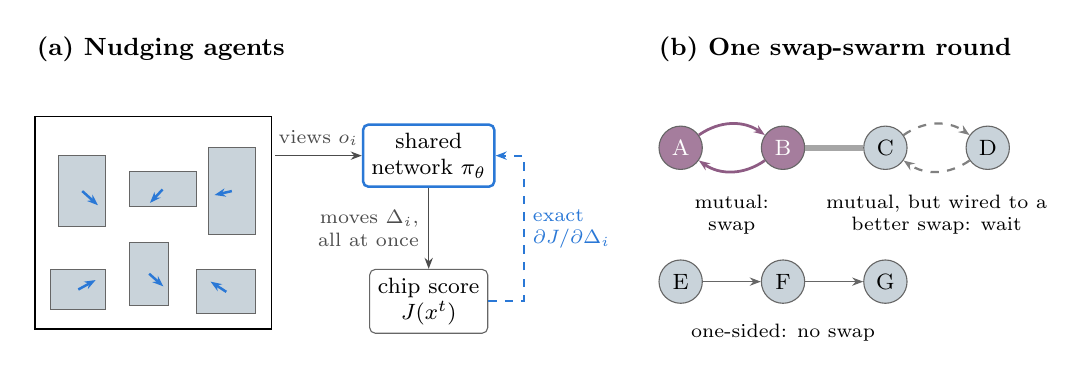
\begin{tikzpicture}[font=\footnotesize, >={Stealth[length=4pt]}]
  % (a) decentralized nudging agents
  \begin{scope}
    \node[font=\small\bfseries, anchor=west] at (-0.1,3.55) {(a) Nudging agents};
    \draw[line width=0.5pt] (0,0) rectangle (3.0,2.7);
    \foreach \x/\y/\w/\h in {0.2/0.25/0.7/0.5, 1.2/0.3/0.5/0.8, 2.05/0.2/0.75/0.55, 0.3/1.3/0.6/0.9, 1.2/1.55/0.85/0.45, 2.2/1.2/0.6/1.1}
      \draw[fill=block, draw=black!60] (\x,\y) rectangle ++(\w,\h);
    \foreach \x/\y/\dx/\dy in {0.55/0.5/0.22/0.12, 1.45/0.7/0.18/-0.16, 2.43/0.47/-0.2/0.13, 0.6/1.75/0.2/-0.18, 1.62/1.77/-0.16/-0.17, 2.5/1.75/-0.22/-0.05}
      \draw[->, agents, line width=0.9pt] (\x,\y) -- ++(\dx,\dy);
    \node[draw=agents, line width=0.9pt, fill=white, rounded corners=2pt, align=center, inner sep=3pt] (net) at (5.0,2.2) {shared\\network $\pi_\theta$};
    \node[draw=black!60, fill=white, rounded corners=2pt, align=center, inner sep=3pt] (J) at (5.0,0.35) {chip score\\$J(x^{t})$};
    \draw[->, black!70] (3.05,2.2) -- node[above, font=\scriptsize]{views $o_i$} (net.west);
    \draw[->, black!70] (net.south) -- node[left, font=\scriptsize, align=right]{moves $\Delta_i$,\\all at once} (J.north);
    \draw[->, agents, dashed, line width=0.8pt] (J.east) -- ++(0.45,0) |- (net.east);
    \node[font=\scriptsize, text=agents, align=left, anchor=west] at (6.2,1.27) {exact\\$\partial J/\partial \Delta_i$};
  \end{scope}
  % (b) swap swarm
  \begin{scope}[xshift=7.9cm]
    \node[font=\small\bfseries, anchor=west] at (-0.1,3.55) {(b) One swap-swarm round};
    \tikzset{m/.style={circle, draw=black!60, fill=block, minimum size=0.55cm, inner sep=0pt}}
    \node[m, fill=swapc!80, text=white] (A) at (0.3,2.3) {A};
    \node[m, fill=swapc!80, text=white] (B) at (1.6,2.3) {B};
    \node[m] (C) at (2.9,2.3) {C};
    \node[m] (D) at (4.2,2.3) {D};
    \node[m] (E) at (0.3,0.6) {E};
    \node[m] (F) at (1.6,0.6) {F};
    \node[m] (G) at (2.9,0.6) {G};
    \draw[swapc, line width=1pt, ->] (A) to[bend left=35] (B);
    \draw[swapc, line width=1pt, ->] (B) to[bend left=35] (A);
    \draw[black!50, line width=0.8pt, dashed, ->] (C) to[bend left=35] (D);
    \draw[black!50, line width=0.8pt, dashed, ->] (D) to[bend left=35] (C);
    \draw[black!35, line width=2pt] (B) -- (C);
    \draw[black!60, ->] (E) -- (F); \draw[black!60, ->] (F) -- (G);
    \node[font=\scriptsize, align=center] at (0.95,1.45) {mutual:\\swap};
    \node[font=\scriptsize, align=center] at (3.55,1.45) {mutual, but wired to a\\better swap: wait};
    \node[font=\scriptsize, align=center] at (1.6,-0.05) {one-sided: no swap};
  \end{scope}
\end{tikzpicture}
\caption{\textbf{(a)} Each macro reads its local view $o_i$, the shared network turns it into a small move $\Delta_i$, and all macros move at once. The design is scored by one differentiable objective $J$, and its gradient tells each macro how its own move changed the score. \textbf{(b)} In a round of the swap swarm, each macro names the same-size macro it would most like to swap with. A and B name each other and swap. C and D also agree, but C is wired to B, whose swap scores higher, so C and D wait. E names F but F names G, so nothing happens.}
\label{fig:overview}
\end{figure}

\subsection{Problem}
A design has $n$ macros with lower-left positions $x_i\in\mathbb{R}^2$, measured in grid cells, and fixed sizes. Each net connects pins at fixed offsets on several macros. The half-perimeter wirelength sums, over nets, the width and height of the box around the net's pins:
\begin{equation}
\hpwl(x) \;=\; \sum_{e\in E}\Big(\max_{p\in e} p_x-\min_{p\in e} p_x\Big) + \Big(\max_{p\in e} p_y-\min_{p\in e} p_y\Big).
\label{eq:hpwl}
\end{equation}
A placement is \emph{legal} if no two macros overlap and all lie on the canvas. Every method starts from the same legal greedy placement $x^0$, in which macros are placed one at a time on the free grid cell that adds the least wirelength (MaskPlace's wire mask used greedily~\citep{lai2022maskplace,shi2023wiremask}). We report the improvement
\begin{equation}
\impr(x) \;=\; 1-\frac{\hpwl(\mathcal{L}(x))}{\hpwl(x^0)},
\label{eq:impr}
\end{equation}
where $\mathcal{L}$ is the legalizer of \S\ref{sec:legalize}. Higher is better. The greedy start has improvement $0$, and a negative value means the method made the placement worse.

\subsection{Agents}
An episode has $T=32$ steps. At each step every macro $i$ computes its view $o_i(x^t)$ and all macros move together:
\begin{equation}
x_i^{t+1} = \mathrm{clip}\big(x_i^t + \Delta_i^t\big),\qquad \Delta_i^t = s\,\tanh\!\big(\mu_\theta(o_i(x^t)) + \sigma_\theta\,\epsilon_i^t\big),\quad \epsilon_i^t\sim\mathcal{N}(0,I).
\label{eq:move}
\end{equation}
$\mu_\theta$ is a two-layer network (64 tanh units per layer) shared by all macros, $s=1$ grid cell limits each move, and the clip keeps macros on the canvas. The noise $\epsilon$ is used in training only. We compare three views, all given relative to the macro and scaled by the canvas size so that one network can run on any design:
\textbf{m0}, the macro's position, size and distance to each canvas edge (8 numbers);
\textbf{m1}, m0 plus the relative position, size and connection weight of its 4 most strongly connected macros (32 numbers);
\textbf{m1all}, m1 plus the weighted mean and spread of the directions to \emph{all} connected macros, their total connection weight and their count (38 numbers).

\subsection{Objective and training}
All agents share the objective
\begin{equation}
J(x) \;=\; \frac{W_\gamma(x)}{W_\gamma(x^0)} \;+\; \lambda_d\,\frac{D(x)}{A} \;+\; \lambda_o\,\frac{\sum_{i<j}\mathrm{area}(i\cap j)}{A},
\label{eq:objective}
\end{equation}
where $W_\gamma$ is a smooth (log-sum-exp) version of~\eqref{eq:hpwl} with $\gamma=1$ cell, $D$ is the area by which grid bins exceed 95\% density plus the area outside the canvas, $A$ is the total macro area, $\lambda_d=1$, and $\lambda_o$ weights the overlap between pairs of macros. The training loss is the mean of $J$ over the $T{+}1$ placements of an episode. We back-propagate it through~\eqref{eq:move} and cut the gradient every $H=8$ steps, as in SHAC~\citep{xu2022shac} but without a value function. Each $\Delta_i$ receives the exact derivative of the shared objective. A training run has 100 episodes, uses Adam~\citep{kingma2015adam} with learning rate $10^{-3}$, and takes about 30\,s on a laptop GPU.

\subsection{Legalization}\label{sec:legalize}
Gradient-based methods can end with overlapping macros, so every result goes through the same legalizer $\mathcal{L}$ before it is scored. The \emph{repair} step rounds positions to the grid, then takes macros from largest to smallest and moves each overlapping one to the free position, among its 256 nearest, that adds the least wirelength. The \emph{spread} step runs 300 steps of gradient descent on the overlap area alone, moving each macro at most 0.25 cells per step, so that neighbours make room instead of one macro jumping far. $\mathcal{L}$ runs the repair once with and once without spreading and keeps the legal result with the lower HPWL. A placement that is already legal is not changed. Section~\ref{sec:dense} explains why the spread step is needed.

\subsection{Swap swarm}\label{sec:swarm-method}
Exchanging two macros of the same size keeps a placement legal. Algorithm~\ref{alg:swarm} describes one round. Each macro scores a swap with each of its $k$ nearest same-size macros and names the best. A swap is agreed when two macros name each other. Two agreed swaps that share a wire were each scored as if the other did not happen, so a swap only goes ahead if its score is higher than that of every agreed swap it shares a wire with. Every decision uses only a macro's candidates and the macros it is wired to. We test two ways to score a swap. The \emph{exact} score $g_{ij}$ is the change in HPWL of the nets on $i$ and $j$. The \emph{learned} score $\hat g_\phi(o_i,o_j,x_j-x_i)$ comes from a network the size of the policy that sees only the agents' view. It is trained on adaptec1 to predict $g_{ij}$ (Appendix~\ref{app:judge}).

\begin{algorithm}[t]
\caption{One round of the swap swarm. Every step runs on all macros in parallel.}\label{alg:swarm}
\begin{algorithmic}[1]
\Require placement $x$; candidates per macro $k$; judge $g$; threshold $\tau$
\For{each macro $i$ \textbf{in parallel}}
  \State $C_i \gets$ the $k$ nearest macros with the same footprint as $i$
  \State $j_i^\star \gets \arg\max_{j\in C_i} g_{ij}(x)$; \ \textbf{if} $g_{ij_i^\star}(x)\le\tau$ \textbf{then} $j_i^\star\gets\varnothing$
\EndFor
\State $P\gets\{(i,j): j_i^\star=j \wedge j_j^\star=i\}$ \Comment{mutual consent}
\For{each $(i,j)\in P$ \textbf{in parallel}}
  \State keep $(i,j)$ unless an $(a,b)\in P$ wired to $\{i,j\}$ has a higher score $g_{ab}{+}g_{ba}$ \Comment{ties by index}
\EndFor
\State exchange the positions of every kept pair, simultaneously
\end{algorithmic}
\end{algorithm}

% ------------------------------------------------------------------------------------------------
\section{Experimental Setup}\label{sec:setup}

\begin{table}[tbp]
\centering
\caption{Designs. On each design, the first 128 macros are placed on a $224\times224$ grid. Policies are trained on adaptec1. bigblue1 and ariane133 are used only to test transfer.}
\label{tab:benchmarks}
\small
\begin{tabular}{@{}llccl@{}}
\toprule
Design & Source & Macros placed & Canvas covered & Macro shapes \\
\midrule
adaptec1 & ISPD 2005~\citep{nam2005ispd} & 128 & $28.6$\% & varied \\
bigblue1 & ISPD 2005~\citep{nam2005ispd} & 128 & $3.5$\% & thin, varied \\
ariane133 & Ariane RISC-V~\citep{zaruba2019ariane,cheng2023assessment} & 128 & $50.0$\% & 128 identical SRAMs \\
\bottomrule
\end{tabular}
\end{table}

\paragraph{Designs.} Table~\ref{tab:benchmarks} lists the three designs. The main difference between them is how full the canvas is: bigblue1 is almost empty, and identical SRAM blocks cover half of ariane133.

\paragraph{Baselines and controls.}
\textbf{Adam}~\citep{kingma2015adam} minimizes~\eqref{eq:objective} directly over the 256 coordinates for 2000 steps (learning rate 0.05), with the same clip and legalizer. It answers Q3.
The \textbf{pull rule} has no learning: every step, each macro moves one cell toward the weighted centre of its 4 most connected macros. It shows what an obvious local rule achieves.
The \textbf{swap search} repeatedly makes the single same-size swap that reduces HPWL the most, until no swap helps. It shows what small continuous moves cannot reach.
\textbf{Random jitter} adds Gaussian noise with a standard deviation of one cell to the greedy start and legalizes it. It shows how much the legalizer alone can change the result.
\textbf{Simulated annealing} starts from the same greedy placement and proposes, with equal probability, a swap of two equal-footprint macros or a shift of one macro into free space within a shrinking window. Both moves keep the placement legal, so annealing is scored on its own output with no legalizer. The temperature is steered to a target acceptance rate that falls from 30\% to 1\%, and the last 10\% of the budget runs at zero temperature from the best placement found. We tuned the acceptance target, the share of swaps and the length of that tail on adaptec1 at a 30\,s budget (12 configurations, best kept), then used one setting on all three designs. Annealing answers the question a reader asks first, because it makes the same move as our swarm.
\textbf{The parallel annealer} is our swarm with that temperature. Each round, a macro proposes a random same-footprint exchange or, with equal probability, a shift into free space within a shrinking window, and accepts its own proposal by the Metropolis rule; mutual consent and the conflict rule are unchanged. Proposals that touch the same macro or the same free area are resolved by keeping the better one. Because many moves are applied at once after local checks only, every round is then verified against the whole grid and dropped if it would leave two macros overlapping. That check is cheap insurance rather than a frequent correction: over \nVerifiedRounds{} instrumented rounds across the three designs it fired on \nRevertedRounds{} of them, and every run we report is legal. It uses the annealer's own temperature schedule and starts from the placement the greedy swarm reaches, inside the same total budget.

\paragraph{Reporting.} Every number in this paper is the improvement~\eqref{eq:impr} of a legalized placement over the greedy start of the same design, in percent. Methods without randomness (pull rule, swap search, swap swarm with the exact score) are run once. Adam is run once and evaluated every 100 steps. Each learned policy is trained with 3 seeds and evaluated every 5 episodes. For Adam and for each seed, we report the median of the last 5 evaluations, never the best one, and tables give the mean and standard deviation over the 3 seeds. Random jitter uses 5 noise seeds. \emph{Transfer} runs the adaptec1 policy for one episode, without noise or retraining, on another design. All values are computed from the stored runs by one script (Appendix~\ref{app:repro}).

% ------------------------------------------------------------------------------------------------
\section{Results}\label{sec:results}

\begin{table}[tbp]
\centering
\caption{Main results: improvement~\eqref{eq:impr} in \%, higher is better. Learned methods: mean\,$\pm$\,std over 3 seeds. Jitter: mean\,$\pm$\,std over 5 noise seeds. Other methods are single runs. Best value per design in bold. $^\dagger$On bigblue1 and ariane133, the policy trained on adaptec1 is applied without retraining. $^\ast$One policy seed.}
\label{tab:main}
\small
\begin{tabular}{@{}lccc@{}}
\toprule
Method & adaptec1 & bigblue1 & ariane133 \\
 & \small (training) & \small (unseen) & \small (unseen) \\
\midrule
\multicolumn{4}{@{}l}{\emph{No learning}} \\
\quad Random jitter + legalize (control) & $-2.6\,\pm\,2.5$ & $-1.6\,\pm\,7.0$ & $-2.1\,\pm\,0.1$ \\
\quad Pull toward partners & $+11.0$ & $+15.5$ & $+2.7$ \\
\quad Swap search (central) & $+18.1$ & $\mathbf{+44.4}$ & $+33.8$ \\
\multicolumn{4}{@{}l}{\emph{Direct optimization}} \\
\quad Adam, $\lambda_o=0$ & $+16.7$ & $+8.2$ & $+0.6$ \\
\quad Adam, $\lambda_o=3$ & $+2.0$ & $+4.1$ & $-1.6$ \\
\multicolumn{4}{@{}l}{\emph{Decentralized agents (ours)}} \\
\quad Nudging agents, m1all, $\lambda_o=3$$^\dagger$ & $+7.0\,\pm\,0.1$ & $+1.9\,\pm\,1.4$ & $-6.6\,\pm\,2.9$ \\
\quad Swap swarm, exact judge & $+18.1$ & $\mathbf{+44.4}$ & $\mathbf{+35.3}$ \\
\quad Nudging agents, then swap swarm$^{\dagger\ast}$ & $\mathbf{+25.8}$ & $+38.8$ & $+27.8$ \\
\bottomrule
\end{tabular}
\end{table}

Table~\ref{tab:main} gives the main results. The rest of this section explains them.

\subsection{Agents exploit the legalizer unless overlap is penalized}\label{sec:measure}

\begin{figure}[tbp]
\centering
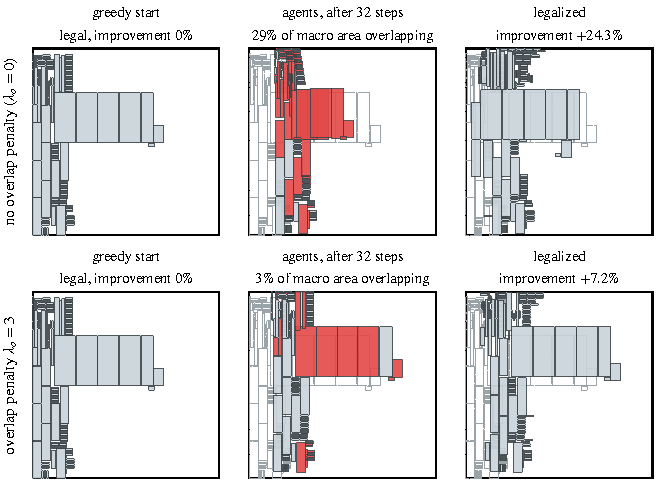
\includegraphics[width=\textwidth]{figures/placements.pdf}
\caption{adaptec1, placements produced by the best evaluation of seed 0 (so the top-right value is higher than the median reported in the text). Red macros overlap at least one other macro, even slightly; dashed outlines show the greedy start. \textbf{Top:} m1 view without an overlap penalty; the agents pile macros on top of each other and the legalizer rebuilds the placement. \textbf{Bottom:} m1all view with $\lambda_o=3$; the agents make small moves that the legalizer barely changes.}
\label{fig:placements}
\end{figure}

\begin{figure}[tbp]
\centering
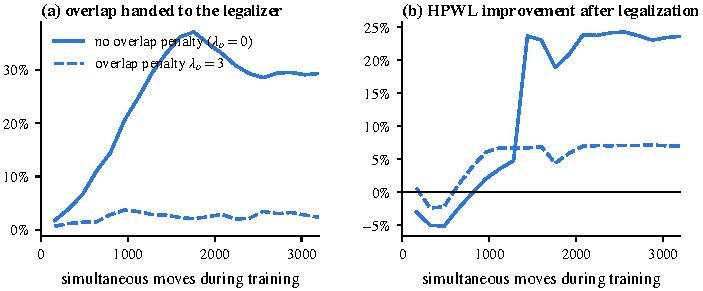
\includegraphics[width=\textwidth]{figures/dynamics.pdf}
\caption{Training on adaptec1 (seed 0, evaluated every 5 episodes; m1 view for $\lambda_o=0$, m1all view for $\lambda_o=3$). \textbf{(a)} Share of macro area that overlaps before legalization. \textbf{(b)} Improvement after legalization. Without the overlap penalty, overlap keeps growing and the result jumps between consecutive evaluations.}
\label{fig:dynamics}
\end{figure}

We first trained the agents with the density term only ($\lambda_o=0$). They learned to push macros onto each other and let the legalizer find legal positions (Fig.~\ref{fig:placements}, top). One evaluation of one seed reached \nFirstRunBest{}, but the median over the last evaluations, averaged over three seeds, is \nFirstRunMedian{}, and the three seeds differ by up to \nNoPenaltySpreadPts{} points. The legalized result also jumps from one evaluation to the next (Fig.~\ref{fig:dynamics}b), so a single best evaluation says little. With an overlap weight of $\lambda_o=3$, overlap stays near 3\%, the result is stable, and the three seeds give \nPenaltyThree{} with a standard deviation of \nPenaltyThreeSdPts{} points (Table~\ref{tab:ablation}). A weight of 10 stops the agents from moving. We use $\lambda_o=3$ from here on.

\subsection{Q1, Q2 and Q4: what a macro needs to see, and transfer}\label{sec:sight}

\begin{figure}[tbp]
\centering
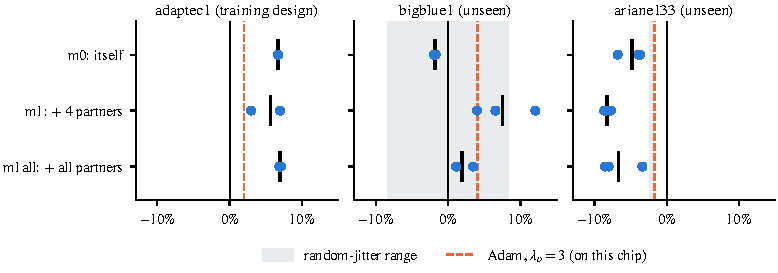
\includegraphics[width=\textwidth]{figures/sight.pdf}
\caption{Improvement per view ($\lambda_o=3$; dots are seeds, bars are means). The orange line is Adam run directly on that design. The grey band is the range of the random-jitter control. A transferred result inside it cannot be told apart from noise.}
\label{fig:sight}
\end{figure}

\textbf{Q1.} The agents improve their training design by \nAgentsHome{} with the m1all view, and the three seeds agree to within a fraction of a point.

\textbf{Q2.} On adaptec1 the view hardly matters: m0 reaches \nAgentsHomeMzero{} and m1 \nAgentsHomeMone{} (Fig.~\ref{fig:sight}). A macro that knows only its own position can still learn where to move on the one design it is trained on. The views differ on other designs. On bigblue1, m0 gives \nTransferMzeroBigblue{} and m1 gives \nTransferMoneBigblue{}, so what carries over is knowing where one's connected macros are.

\textbf{Q4.} That transfer is not larger than noise. Random jitter alone gives up to \nJitterBigblueMax{} on bigblue1, and on ariane133 every transferred policy makes the placement worse (\nTransferWorstAriane{} to \nTransferBestAriane{}). Two methods from neural cellular automata~\citep{mordvintsev2020growing}, moving a random half of the macros each step and training from noisy starting placements, reduce overfitting to adaptec1 but do not change this conclusion (Table~\ref{tab:ablation}).

\begin{table}[tbp]
\centering
\caption{Ablations: improvement in \%, mean\,$\pm$\,std over 3 seeds. $^\ddagger$Share of macro area overlapping before legalization. $^\S$bigblue1 is also a training design here. Policies in the first block were transferred to bigblue1 only.}
\label{tab:ablation}
\small
\begin{tabular}{@{}lcccc@{}}
\toprule
Variant (m1all unless noted) & adaptec1 & overlap$^\ddagger$ & bigblue1 & ariane133 \\
\midrule
\multicolumn{5}{@{}l}{\emph{Overlap penalty and step schedule}} \\
\quad m1, $\lambda_o=0$ & $+6.5\,\pm\,14.9$ & $31$\% & $+6.8\,\pm\,8.4$ & -- \\
\quad $\lambda_o=0$ & $-0.3\,\pm\,11.5$ & $38$\% & $+4.8\,\pm\,3.2$ & -- \\
\quad $\lambda_o=3$ & $+6.8\,\pm\,0.2$ & $3$\% & $+0.2\,\pm\,4.4$ & -- \\
\quad $\lambda_o=10$ & $-0.3\,\pm\,0.3$ & $1$\% & $+1.9\,\pm\,1.3$ & -- \\
\quad steps $16\to1$, $\lambda_o=0$ & $+0.2\,\pm\,9.9$ & $63$\% & $+11.9\,\pm\,1.3$ & -- \\
\quad steps $16\to1$, $\lambda_o=10$ & $-39.9\,\pm\,5.9$ & $15$\% & $+5.9\,\pm\,6.2$ & -- \\
\midrule
\multicolumn{5}{@{}l}{\emph{Swarm rules and generalization ($\lambda_o=3$)}} \\
\quad none (reference) & $+7.0\,\pm\,0.1$ & $3$\% & $+1.9\,\pm\,1.4$ & $-6.6\,\pm\,2.9$ \\
\quad alignment $a=0.5$ & $-0.9\,\pm\,0.7$ & $2$\% & $-0.5\,\pm\,2.1$ & $-2.3\,\pm\,0.2$ \\
\quad alignment $a=0.9$ & $0.0\,\pm\,0.7$ & $1$\% & $+1.9\,\pm\,0.7$ & $-1.6\,\pm\,0.5$ \\
\quad random half of macros move & $-1.3\,\pm\,1.0$ & $2$\% & $+8.6\,\pm\,3.4$ & $-2.2\,\pm\,0.2$ \\
\quad noisy starts ($\sigma=4$ cells) & $+1.7\,\pm\,0.3$ & $9$\% & $+6.6\,\pm\,3.7$ & $-3.1\,\pm\,0.8$ \\
\quad noisy starts + trained on bigblue1$^\S$ & $-1.3\,\pm\,0.9$ & $10$\% & $+2.8\,\pm\,3.2$ & $-2.1\,\pm\,0.7$ \\
\bottomrule
\end{tabular}
\end{table}

\subsection{Alignment from swarm models removes the gain}
Our objective already contains two of the three boids rules~\citep{reynolds1987flocks}. The wirelength term pulls connected macros together (cohesion) and the overlap penalty keeps them apart (separation). We added the third, alignment: a macro's move becomes $(1-a)\Delta_i$ plus $a$ times the weighted mean of its connected macros' moves. With $a=0.9$ the improvement on adaptec1 drops to about zero (\nAlignHome{}, Table~\ref{tab:ablation}). Wirelength only falls when connected macros move \emph{relative} to each other, and alignment makes them move together, so the wires inside a group keep their length. Alignment could help a group travel far across the canvas, but moves of at most one cell per step do not allow that.

\subsection{Why the dense design defeated every method}\label{sec:dense}

\begin{figure}[tbp]
\centering
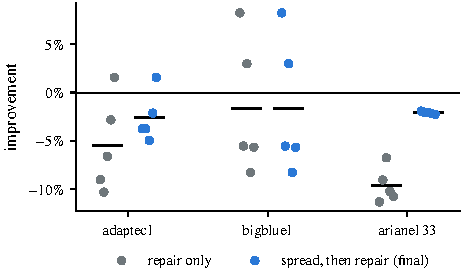
\includegraphics[width=0.6\textwidth]{figures/jitter.pdf}
\caption{Random-jitter control: the greedy start plus noise of one cell, legalized (5 noise seeds; bars are means). With the repair alone, ariane133 loses about 10\%. Spreading first reduces the loss to about 2\%. bigblue1 is unchanged, because there the final legalizer always keeps the repair-only result.}
\label{fig:jitter}
\end{figure}

With the repair-only legalizer, every method made ariane133 worse, including Adam, whose placement before legalization was \nAdamRawAriane{} better than the start. Identical blocks cover half of ariane133, so the nearest free space is usually far away. After one cell of noise, the repair moved macros \nMoveOldAriane{} cells on average and lost \nJitterArianeOld{} (Fig.~\ref{fig:jitter}). Adding the spread step reduces this to \nMoveNewAriane{} cells and \nJitterArianeNew{}, and Adam on ariane133 then reaches \nAdamZeroAriane{}. All results in this paper use the final legalizer. Even with it, gradient-based methods gain almost nothing on ariane133, while the swap search gains \nSwapAriane{}.

\subsection{Q3: agents against direct optimization}\label{sec:q3}

\begin{figure}[tbp]
\centering
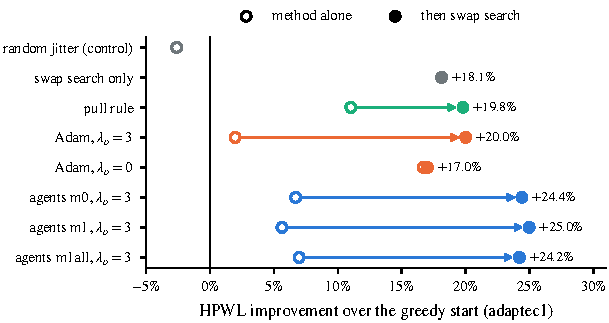
\includegraphics[width=0.78\textwidth]{figures/q3.pdf}
\caption{adaptec1: each method alone (hollow circle) and followed by the swap search (filled circle). Learned methods are means over 3 seeds; the swap search is applied to the last evaluated placement of each seed.}
\label{fig:q3}
\end{figure}

With the same objective ($\lambda_o=3$), the agents do better than Adam: \nAgentsHome{} against \nAdamThreeHome{}. Adam with $\lambda_o=0$ reaches \nAdamZeroHome{}, however, and the swap search reaches \nSwapHome{}, both more than the agents. Most of the slack in the greedy start is in \emph{which} macro sits in which slot. Fixing that requires two blocks to trade places, and small continuous moves cannot do so without passing through an overlap that the penalty forbids. The agents' moves and the swaps do combine on the training design. Running the swap search after the agents gives \nAgentsPlusSwaps{} (m1), more than any other method followed by swaps (at most \nAdamPlusSwapsBest{}; Fig.~\ref{fig:q3}). On unseen designs, the swap search alone does better than any transferred policy, with or without swaps afterwards.

\subsection{Agents that swap}\label{sec:swarm}

\begin{figure}[tbp]
\centering
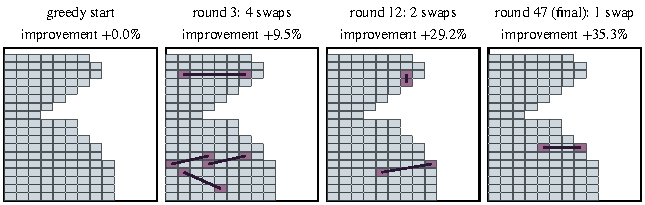
\includegraphics[width=\textwidth]{figures/swarm_frames.pdf}\\[2pt]
{\small (a) Rounds of the swap swarm on ariane133 (exact score, all same-size candidates). Purple macros swapped in that round and are linked to their partner.}\\[6pt]
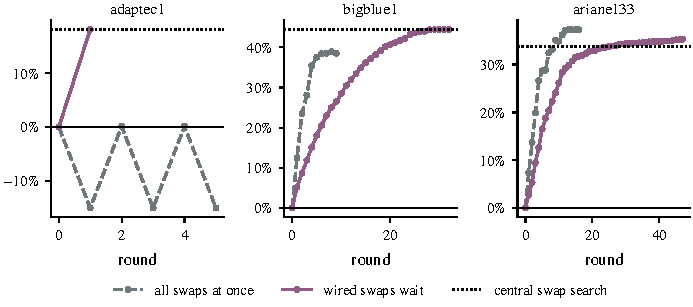
\includegraphics[width=\textwidth]{figures/swarm_trace.pdf}\\[2pt]
{\small (b) Improvement after each round. The dotted line is the central swap search.}
\caption{The swap swarm. On ariane133 it stops after \nSwarmRoundsAriane{} rounds and \nSwarmSwapsAriane{} swaps. Without the conflict rule, adaptec1's four large macros, which share wires, swap back and forth, and the design ends at \nSwarmAtOnceHome{}. Animations are in the supplementary material.}
\label{fig:swarm}
\end{figure}

\begin{table}[tbp]
\centering
\caption{Swap swarm variants: improvement in \%. Exact-score rows are single runs. Learned rows: mean\,$\pm$\,std over 3 seeds; the last learned row pools 6 runs (m1 and m1all).}
\label{tab:swarm}
\small
\begin{tabular}{@{}llccc@{}}
\toprule
Judge & Variant & adaptec1 & bigblue1 & ariane133 \\
\midrule
--- & central swap search (reference) & $+18.1$ & $+44.4$ & $+33.8$ \\
\midrule
exact & all agreed swaps at once & $-15.1$ & $+38.5$ & $+37.3$ \\
exact & wired swaps wait (Alg.~\ref{alg:swarm}) & $+18.1$ & $+44.4$ & $+35.3$ \\
exact & wired swaps wait, 8 nearest candidates & $+18.1$ & $+27.8$ & $+15.5$ \\
\midrule
learned & view m0 & $0.0\,\pm\,0.0$ & $0.0\,\pm\,0.0$ & $0.0\,\pm\,0.0$ \\
learned & view m1 & $+12.0\,\pm\,10.4$ & $-17.4\,\pm\,19.0$ & $-0.6\,\pm\,0.6$ \\
learned & view m1all & $+6.0\,\pm\,10.4$ & $-2.2\,\pm\,3.0$ & $+0.6\,\pm\,0.6$ \\
learned & m1, m1all, also trained on bigblue1 & -- & -- & $+0.9\,\pm\,1.1$ \\
\midrule
exact & after the agents' nudges & $+25.8$ & $+38.8$ & $+27.8$ \\
\bottomrule
\end{tabular}
\end{table}

With the exact score and the conflict rule, the swap swarm matches the central swap search on adaptec1 and bigblue1 and does slightly better on ariane133, \nSwarmAriane{} against \nSwapAriane{} (Table~\ref{tab:swarm}). It also needs fewer rounds (\nSwarmRoundsAriane{}) than the central search needs sequential swaps. The conflict rule is necessary: without it, swaps that share wires undo each other and adaptec1 ends at \nSwarmAtOnceHome{} (Fig.~\ref{fig:swarm}b). Candidates must also be chosen widely. With only the 8 nearest same-size macros as candidates, ariane133 reaches \nSwarmKeightAriane{}, because the best exchange partner is rarely next door.

Learning the swap score gives the same picture as learning the moves. With the m0 view, the learned score never produces a useful swap. With m1 or m1all it finds the three swaps that matter on adaptec1 for some seeds, but it does not help on the other designs, even when trained on two of them (ariane133: \nLearnedTwoChipsAriane{}). The best result on adaptec1, \nNudgeSwapHome{}, comes from running the agents' moves first and the swap swarm second. On the other designs the agents' moves lower the final result.

\subsection{Cost: annealing and wall clock}\label{sec:cost}

\begin{figure}[tbp]
\centering
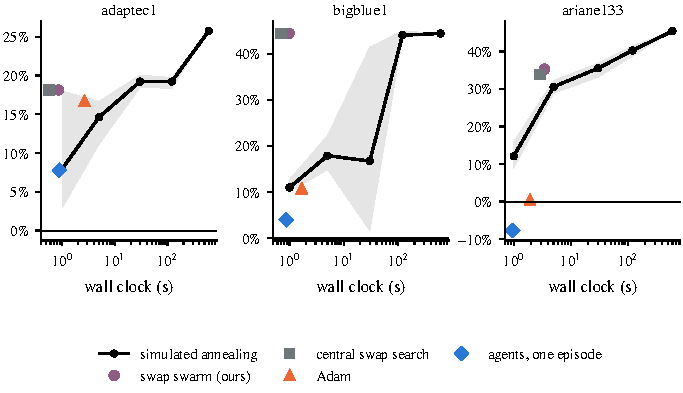
\includegraphics[width=\textwidth]{figures/time.pdf}
\caption{What each method reaches against the time it needs (log scale). The black line is simulated annealing at five budgets and the purple line is our parallel annealer at three, each with a band spanning its seeds. Markers are single runs of the other methods at their measured wall clock, including compilation. The purple line flattens while the black one is still rising: the temperature removes the swarm's early stop, but the search still saturates first.}
\label{fig:time}
\end{figure}

\begin{table}[tbp]
\centering
\caption{Simulated annealing by time budget, against our methods at the wall clock they need. Improvement in \%, mean\,$\pm$\,std over 3 annealing seeds (1 seed at 600\,s).}
\label{tab:anneal}
\small
\begin{tabular}{@{}lccc@{}}
\toprule
Method (time budget) & adaptec1 & bigblue1 & ariane133 \\
\midrule
\multicolumn{4}{@{}l}{\emph{Simulated annealing, 3 seeds (600\,s: 1 seed)}} \\
\quad 1\,s & $+7.9\,\pm\,8.7$ & $+11.0\,\pm\,1.5$ & $+12.1\,\pm\,3.5$ \\
\quad 5\,s & $+14.6\,\pm\,3.0$ & $+17.9\,\pm\,3.8$ & $+30.6\,\pm\,1.7$ \\
\quad 30\,s & $+19.2\,\pm\,0.8$ & $+16.7\,\pm\,21.6$ & $+35.5\,\pm\,2.1$ \\
\quad 120\,s & $+19.2\,\pm\,0.8$ & $+44.0\,\pm\,0.8$ & $+40.3\,\pm\,1.4$ \\
\quad 600\,s & $+25.7$ & $+44.4$ & $+45.4$ \\
\midrule
\multicolumn{4}{@{}l}{\emph{Ours, at the wall clock each one needs}} \\
\quad swap swarm & $+18.1$ \small (0.8\,s) & $+44.4$ \small (1.0\,s) & $+35.3$ \small (3.5\,s) \\
\quad agents, then swap swarm & $+25.8$ \small (1.7\,s) & $+38.8$ \small (1.9\,s) & $+27.8$ \small (4.5\,s) \\
\midrule
\multicolumn{4}{@{}l}{\emph{Parallel annealer, warm-started from the swarm, 3 seeds}} \\
\quad 30\,s & $+18.5\,\pm\,0.6$ & $+44.5\,\pm\,0.1$ & $+35.6\,\pm\,0.1$ \\
\quad 120\,s & $+24.6\,\pm\,0.8$ & $+45.2\,\pm\,0.0$ & $+43.1\,\pm\,2.3$ \\
\quad 600\,s & $+24.9\,\pm\,0.7$ & $+45.7\,\pm\,0.6$ & $+45.3\,\pm\,1.6$ \\
\bottomrule
\end{tabular}
\end{table}

\begin{table}[tbp]
\centering
\caption{Wall clock in seconds, including JAX compilation, and the result reached. One machine: an RTX 3050 laptop GPU, with annealing single-threaded on the CPU.}
\label{tab:runtime}
\small
\begin{tabular}{@{}lcccccc@{}}
\toprule
& \multicolumn{2}{c}{adaptec1} & \multicolumn{2}{c}{bigblue1} & \multicolumn{2}{c}{ariane133} \\
\cmidrule(lr){2-3}\cmidrule(lr){4-5}\cmidrule(lr){6-7}
Method & s & result & s & result & s & result \\
\midrule
central swap search & 0.6 & $+18.1$ & 0.7 & $+44.4$ & 2.9 & $+33.8$ \\
swap swarm (ours) & 0.8 & $+18.1$ & 1.0 & $+44.4$ & 3.5 & $+35.3$ \\
agents, one episode & 0.9 & $+7.8$ & 0.9 & $+4.0$ & 1.0 & $-7.7$ \\
pull rule & 2.3 & $+11.0$ & 1.1 & $+15.5$ & 1.3 & $+2.7$ \\
Adam, 2000 steps & 2.6 & $+16.7$ & 1.7 & $+10.7$ & 1.9 & $+0.4$ \\
simulated annealing, 30\,s & 30 & $+19.2$ & 30 & $+16.7$ & 30 & $+35.5$ \\
simulated annealing, 600\,s & 600 & $+25.7$ & 600 & $+44.4$ & 600 & $+45.4$ \\
\midrule
\multicolumn{7}{@{}l}{\emph{Loading the netlist and building the greedy start, paid by every method}} \\
greedy start & 5.1 & --- & 3.2 & --- & 2.6 & --- \\
\bottomrule
\end{tabular}
\end{table}

Table~\ref{tab:anneal} and Fig.~\ref{fig:time} put every method on one time axis, and Table~\ref{tab:runtime} gives the measured wall clock.

\textbf{At equal time, the swarm is ahead.} Annealing given one second reaches \nAnnealHomeShort{} on adaptec1, while the swap swarm reaches \nSwarmHome{} in \nSwarmSecondsAdaptec{} and the agents followed by the swarm reach \nNudgeSwapHome{} in \nSwarmSecondsSum{}. Annealing needs about 30\,s to match the swarm on adaptec1 (\nAnnealHomeThirty{}) and about 120\,s on bigblue1.

\textbf{Given far more time, annealing wins.} At 600\,s it reaches \nAnnealHomeLong{} on adaptec1, \nAnnealBigblueLong{} on bigblue1 and \nAnnealArianeLong{} on ariane133, the last well above the swarm's \nSwarmAriane{}. The swarm stops when no macro wants to trade, which is a local optimum of its move set, while annealing accepts uphill moves and keeps going.

\textbf{A temperature removes the swarm's early stop, but not its saturation.} At a 120\,s budget the parallel annealer is ahead of the sequential one on all three designs: \nParallelHome{} against \nAnnealHomeMid{} on adaptec1, \nParallelBigblue{} against \nAnnealBigblueMid{} on bigblue1, and \nParallelAriane{} against \nAnnealArianeMid{} on ariane133 (Table~\ref{tab:anneal}). The gain over the swarm it starts from is largest where the swarm stopped earliest: on ariane133 it turns \nSwarmAriane{} into \nParallelAriane{}. At 600\,s the picture is mixed. It still leads on bigblue1 (\nParallelBigblueLong{} against \nAnnealBigblueLong{}), is level on ariane133 (\nParallelArianeLong{} against \nAnnealArianeLong{}), and is behind on adaptec1 (\nParallelHomeLong{} against \nAnnealHomeLong{}), where it gains almost nothing between the two budgets. The temperature removes the hard stop at a local optimum of the exchange move, but every proposal still comes from a macro that only considers partners of its own footprint, and the search converges earlier than the sequential annealer's. The 600\,s annealing column is a single seed, so those three comparisons rest on one run each. Two choices decide whether it works at all. It must start from the swarm's answer rather than the greedy placement, because it keeps the best placement it has seen and therefore cannot end below its start; cold-started it was unreliable on the sparse design. And its macros must propose a \emph{random} same-size partner rather than their best one: proposing the best partner is what the greedy swarm already does, it re-proposes the same blocked exchange every round, and scanning every candidate to do so costs roughly four times the wall clock per round. At the 30\,s budget our figure is not meaningful on adaptec1, because the GPU compilation our implementation pays on its first call falls inside the budget.

\textbf{Read the speed comparison with care.} The two implementations do not use the same hardware: the swarm scores all candidate swaps in parallel on a GPU, and the annealer is a single-threaded NumPy loop proposing one move at a time. A hardware-independent measure is how many candidate moves each one scores. On ariane133 the swarm scores \nSwarmEvalsAriane{} candidates in total, and annealing proposes \nAnnealMovesAriane{} in 120\,s, by which point it is already ahead (\nAnnealArianeMid{} against \nSwarmAriane{}). On adaptec1 the ordering reverses: the swarm needs \nSwarmEvalsAdaptec{} evaluations for \nSwarmHome{}, two orders of magnitude fewer than annealing spends before passing it. The swarm is thus more efficient per evaluation on the sparse and mixed designs and less efficient on the dense one, and its wall-clock advantage comes from evaluating a whole round at once.

% ------------------------------------------------------------------------------------------------
\section{Discussion}

\paragraph{What the agents learned.} On the design they train on, the agents learn a small, repeatable improvement. The view barely matters there, because even m0 can learn the one design. Seeing connected macros is needed for any transfer, but the transfer we measured is no larger than noise. The agents are most useful before a swap search, and less useful as a rule for new designs.

\paragraph{Why swaps work and learned swap scores do not.} Each macro can compute the exact effect of a swap from its own nets, and the conflict rule stops wired neighbours from acting on conflicting plans. The learned score only approximates a value that the macro can compute exactly. That it does not transfer matches the result for moves: features learned on one design do not describe another well.

\paragraph{What the annealing comparison changes.} The swarm is not a better search than annealing; it is a faster one per unit of wall clock, and it stops earlier. Both use the same exchange move, and annealing's willingness to accept a worse placement is what lets it pass the swarm given enough time, especially on the dense design where good exchanges are rare and have to be reached through worse intermediate states. The consequence is to give the swarm the same ability: accept a proposed exchange with a probability set by a temperature, keeping mutual consent and the conflict rule, which turns it into a parallel annealer rather than a parallel descent. That is what the last row block of Table~\ref{tab:anneal} measures. It holds at moderate budgets: the swarm no longer stops at the local optimum of its move set, and at 120\,s it is ahead of the sequential annealer on every design. It does not hold indefinitely, because the parallel annealer saturates by 600\,s while the sequential one is still improving. Refusing to move uphill was one limit and the temperature removes it; the other is the move set itself, since a macro only ever considers partners of its own footprint.

\paragraph{Evaluation.} Two early conclusions were wrong because of the legalizer: a first result of \nFirstRunBest{}, and the impression that ariane133 could not be improved. Any placer evaluated after legalization can be misled in the same way. We suggest reporting a random-jitter range, a swap-search baseline, and medians over several seeds and evaluations.

\paragraph{Limitations.} We use three designs and 128 macros per design, and measure only wirelength, because the benchmarks include no timing data. Adam is a weaker baseline than a full analytical placer such as DREAMPlace~\citep{lin2019dreamplace}. The timing comparison is bound to our implementations: a compiled, multi-threaded annealer would propose many more moves per second than our NumPy loop, which would narrow or remove the wall-clock advantage we measure. Swaps are limited to macros of the same size. The agents are trained without a value function. Natural next steps are swaps between macros of different sizes, using the agents and swaps after a stronger initial placer, and a comparison with DREAMPlace on more designs.

% ------------------------------------------------------------------------------------------------
\section{Conclusion}
Macros acting as identical agents with local information can improve a placement. Through small moves the gain is modest and does not transfer to other designs. Through swaps agreed between pairs, with a local rule for conflicts, they do as well as a central swap search, and better than simulated annealing at equal wall clock. Annealing overtakes a swarm that only moves downhill; letting each macro accept an uphill exchange by the Metropolis rule delays that crossing by an order of magnitude in time, without giving any macro a wider view. In both cases, learned decisions did not generalize, while exactly computed ones did. Controls for the legalizer were needed to reach these conclusions.

\small
\bibliographystyle{plainnat}
\bibliography{refs}
\normalsize

% ------------------------------------------------------------------------------------------------
\clearpage
\appendix
\section{Hyperparameters}\label{app:hyper}
\begin{table}[h]
\centering
\small
\begin{tabular}{@{}ll@{}}
\toprule
Setting & Value \\
\midrule
Grid, macros, canvas & $224\times224$; first 128 macros; core area (whole die for ariane133) \\
Episode & $T=32$ simultaneous steps, $|\Delta_i|\le1$ cell per axis \\
Policy & 2 hidden layers of 64 tanh units; initial $\log\sigma=-1.5$ \\
Objective & $\gamma=1$ cell, target density 0.95, $\lambda_d=1$, $\lambda_o=3$ unless stated \\
Training & 100 episodes, Adam, learning rate $10^{-3}$, gradient-norm clip 1, window $H=8$ \\
Evaluation & every 5 episodes, no noise; median of the last 5 \\
Legalizer & repair over the 256 nearest free positions; spread: 300 steps of $\le0.25$ cells \\
Adam baseline & 2000 steps, learning rate 0.05, evaluated every 100 steps \\
Swap swarm & $k=8$ or all same-size macros as candidates; learned-score threshold $\tau=0.3$ \\
\bottomrule
\end{tabular}
\end{table}

\section{Learned swap score}\label{app:judge}
The learned score $\hat g_\phi$ is a network with two layers of 64 tanh units. Its input is the view of both macros and their relative position. Its target is the exact gain divided by the mean HPWL per macro of the placement, clipped to $[-5,5]$. Training placements are the greedy start, the greedy start after 3 to 60 random same-size swaps, and the placements visited by the exact swap swarm from these starts. This gives \nScorerSamples{} candidate pairs on adaptec1, of which 3 to 4\% reduce HPWL. We train for 30 epochs with Adam and a Huber loss. At run time a macro proposes a swap only if the predicted gain exceeds $\tau=0.3$, because most candidate swaps change nothing and small positive predictions for them are noise.

\section{Reproducibility}\label{app:repro}
\texttt{bash multiagent/run\_all.sh} reruns every experiment in about 45 minutes on a laptop GPU, plus two hours for the fixed time budgets of the two annealers, which should be given an otherwise idle machine because their results are wall clocks. \texttt{python -m multiagent.paper.build} then recomputes every figure, table and number in this paper from the stored runs and compiles it. GPU computations are not bit-for-bit deterministic, so a rerun reproduces the conclusions but not every digit. Animations of the agents and the swap swarm are in \texttt{multiagent/paper/SUPPLEMENTARY.md}.

\end{document}
